\documentclass[11pt]{article}
\usepackage[letterpaper,margin=1in]{geometry}
\usepackage[T1]{fontenc}
\usepackage[utf8]{inputenc}
\usepackage{lmodern}
\usepackage{microtype}
\usepackage{amsmath,amssymb,amsthm,mathtools}
\usepackage{booktabs,longtable,array,tabularx}
\usepackage{enumitem}
\usepackage{xcolor}
\usepackage{graphicx}
\usepackage{listings}
\usepackage{url}
\usepackage{hyperref}
\usepackage[nameinlink,noabbrev]{cleveref}
\usepackage{fancyhdr}
\usepackage{lastpage}

\graphicspath{{../figures/}}
\hypersetup{
  colorlinks=true,
  linkcolor=blue!55!black,
  citecolor=green!35!black,
  urlcolor=blue!65!black,
  pdftitle={The Conway criterion in intuitionistic primitive recursive arithmetic},
  pdfauthor={OpenAI, prepared for Vladimir Reshetnikov},
  pdfsubject={Constructive tiling theory and iPRA formalization plan},
  pdfkeywords={Conway criterion, tiling, iPRA, primitive recursive arithmetic, Lean, torus}
}

\pagestyle{fancy}
\fancyhf{}
\lhead{Conway criterion in iPRA}
\rhead{\thepage/\pageref{LastPage}}
\setlength{\headheight}{14pt}

\newtheorem{theorem}{Theorem}[section]
\newtheorem{lemma}[theorem]{Lemma}
\newtheorem{proposition}[theorem]{Proposition}
\newtheorem{corollary}[theorem]{Corollary}
\theoremstyle{definition}
\newtheorem{definition}[theorem]{Definition}
\newtheorem{construction}[theorem]{Construction}
\newtheorem{example}[theorem]{Example}
\theoremstyle{remark}
\newtheorem{remark}[theorem]{Remark}

\newcommand{\Z}{\mathbb Z}
\newcommand{\Q}{\mathbb Q}
\newcommand{\R}{\mathbb R}
\newcommand{\Torus}{\mathbb T}
\newcommand{\Area}{\operatorname{area}}
\newcommand{\detp}[2]{\det(#1,#2)}
\newcommand{\rev}{\operatorname{rev}}
\newcommand{\PathJ}{\mathcal J}
\newcommand{\trans}[1]{\tau_{#1}}
\newcommand{\half}[1]{H_{#1}}
\newcommand{\code}[1]{\texttt{#1}}
\newcommand{\PRA}{\mathrm{PRAAx}}
\newcommand{\Prf}{\mathrm{Prf}}
\newcommand{\bool}{\mathbf B}

\lstdefinestyle{leanstyle}{
  language={},
  basicstyle=\ttfamily\small,
  columns=fullflexible,
  frame=single,
  breaklines=true,
  showstringspaces=false,
  backgroundcolor=\color{black!2}
}
\lstset{style=leanstyle}

\title{\textbf{The Conway Criterion in Intuitionistic Primitive Recursive Arithmetic}\\[0.5ex]
\large An explicit two-orbit construction and a finite torus-chain proof}
\author{Research packet prepared for Vladimir Reshetnikov}
\date{16 November 2026}

\begin{document}
\maketitle
\begin{abstract}
The Conway criterion is a local symmetry test implying that a topological disk tiles the plane periodically by translations and half-turns.  Its usual proofs describe matching strips or double the tile into a generalized parallelogram or hexagon.  Those pictures correctly identify the construction, but a completely formal proof must still rule out a gap or overlap at the vertices where several boundary arcs meet.

This report gives a finite, constructive proof for rational piecewise-linear disks, the natural arithmetic presentation of polygonal and polyform instances.  If the counterclockwise boundary is split into six paths
\(a,b,c,d,e,f\), with \(a\) translating to the reverse of \(d\) and the other four paths invariant under their endpoint half-turns, define
\[
 t=E-A=D-B,
 \qquad
 u=E+F-B-C,
 \qquad
 H_e(x)=E+F-x.
\]
The explicit family
\[
 T+mt+nu,
 \qquad
 H_e(T)+mt+nu
 \quad (m,n\in\Z)
\]
is shown to be a tiling.  The proof projects the two orbit representatives to the period torus \(\R^2/(\Z t+\Z u)\).  Their oriented boundaries cancel.  After a finite common subdivision they form a nonnegative two-cycle, hence have a constant coverage multiplicity.  An exact open-path shoelace calculation gives
\[
 \det(t,u)=2\Area(T)>0,
\]
so the two representatives have exactly the area of one torus fundamental cell and the constant multiplicity is one.  This simultaneously proves coverage, disjointness of interiors, and nondegeneracy of the period lattice.

Every ingredient is finite: signed rational arithmetic, lists of vertices, a certified triangulation, segment clipping, a dual spanning tree, and bounded sums.  We formulate the resulting number-coded theorem as a quantifier-free universal schema of intuitionistic primitive recursive arithmetic (iPRA), audit the proof for constructive principles, and give a dependency-ordered route to a Lean theorem of type
\[
 ([] : \mathrm{List}(\mathrm{Fm}\;\mathrm{PTm}\;0))\ \vdash[\PRA]\ \varphi_{\rm Conway}.
\]
The packet also contains exact Python reference code, a nonconvex worked example, figures, and an uncompiled Lean blueprint.  The mathematical theorem is proved here; a kernel-checked \(\Prf\,\PRA\) object remains a clearly delimited formalization task.
\end{abstract}

\paragraph{Deliverable status.}
The report proves the finite PL theorem without excluded middle, choice, compactness, or a classical covering-space argument.  The executable companion validates the algebraic and torus certificates of the worked example using exact rational arithmetic.  The Lean files contain no admitted facts, but they are a blueprint rather than a completed formal proof.

\tableofcontents
\clearpage
\section{Statement, representation, and logical scope}
\label{sec:scope}

\subsection{The ordinary geometric criterion}

Let \(T\subseteq\R^2\) be a closed topological disk.  Choose six consecutive boundary points
\[
 A,B,C,D,E,F
\]
in counterclockwise order; adjacent chosen points are allowed to coincide, so an intervening boundary part may be empty.  Write
\[
 a=AB,\quad b=BC,\quad c=CD,\quad d=DE,\quad e=EF,\quad f=FA
\]
for the corresponding oriented boundary paths.  Conway's condition is:
\begin{enumerate}[label=(\roman*)]
\item a translation takes \(A\) to \(E\), \(B\) to \(D\), and the path \(a\) to the path \(ED=\rev(d)\);
\item each of \(b,c,e,f\) is invariant, as an unoriented path, under the half-turn interchanging its endpoints;
\item at least three of \(A,\ldots,F\) are distinct.
\end{enumerate}
The conclusion is that congruent copies of \(T\), obtained using translations and half-turns, tile the plane periodically.  This is the labelled formulation emphasized by Schattschneider~\cite{Schattschneider1980}; it removes the ambiguity in saying merely that two boundary parts are ``parallel.''

The strip proof is geometrically persuasive: translate copies along \(a,d\) to form a strip, rotate a second strip around a midpoint of \(e\) or \(f\), and repeat.  A modern exposition explicitly observes that this description is still vague at the vertices and cites simple connectivity and covering spaces as a repair~\cite[Remark~3.4.4]{Weber2025}.  The purpose of this report is to make that repair finite and arithmetical.

\subsection{Why an arithmetic presentation is needed}

First-order iPRA has natural numbers as objects.  It does not directly quantify over arbitrary subsets of \(\R^2\), arbitrary continuous maps, or an uncountable family of tile copies.  A theorem in iPRA must therefore specify:
\begin{itemize}
\item how a tile and its boundary are number-coded;
\item which finite certificate says that the code is a disk;
\item which primitive-recursive functions produce the proposed tiling certificate; and
\item which bounded, decidable predicate verifies that certificate.
\end{itemize}

The exact theorem proved here uses a \emph{rational piecewise-linear disk}.  After multiplying all coordinates by a common denominator, one may equivalently use integer coordinates.  A disk certificate consists of a finite list of positively oriented triangles with exact edge-incidence data.  The union of the triangles is the tile, their interiors are pairwise disjoint, every interior edge occurs twice with opposite orientations, and the remaining oriented edges form one simple boundary cycle.  The six boundary paths are finite vertex lists along that cycle.  A geometrically empty path is represented by a singleton list.

This covers polygons, polyominoes, polyiamonds, polyhexes, and every exact finite straight-line model normally used in applications of the criterion.  It is also the correct finite kernel for extensions to effectively named curved boundaries: an extension must supply enough modulus and approximation data to reduce the relevant claim to compatible finite PL certificates.  We do not silently identify that stronger represented-analysis theorem with the finite theorem proved below.

\begin{definition}[Normalized PL Conway datum]
A \emph{normalized PL Conway datum} is a positively oriented rational PL disk \(T\), a certified triangulation of \(T\), and six nonempty vertex lists \(a,b,c,d,e,f\) whose concatenation is the oriented boundary cycle, satisfying
\begin{align}
 \trans{t}(a)&=\rev(d), & t&=E-A, \label{eq:ad}\\
 \half{B+C}(b)&=\rev(b), \label{eq:bhalf}\\
 \half{C+D}(c)&=\rev(c), \label{eq:chalf}\\
 \half{E+F}(e)&=\rev(e), \label{eq:ehalf}\\
 \half{F+A}(f)&=\rev(f). \label{eq:fhalf}
\end{align}
Here \(\trans{w}(x)=x+w\), while \(\half{s}(x)=s-x\) is the half-turn whose \emph{doubled center} is \(s\).  Equality of paths means equality after deleting consecutive duplicate vertices and redundant collinear subdivision vertices.
\end{definition}

Using doubled centers avoids division by two.  Every displayed equation is an equality of finite lists of rational points, hence is decidable by cross multiplication.

\subsection{The explicit theorem}

Set
\begin{equation}
  t=E-A,
  \qquad
  u=E+F-B-C,
  \qquad
  R=\half{E+F}.
  \label{eq:periods}
\end{equation}
For \((m,n)\in\Z^2\), define two tile orbits
\begin{equation}
 T^0_{m,n}=T+mt+nu,
 \qquad
 T^1_{m,n}=R(T)+mt+nu.
 \label{eq:tilefamily}
\end{equation}

\begin{theorem}[Finite PL Conway criterion]
\label{thm:mainPL}
For every normalized PL Conway datum:
\begin{enumerate}[label=(\alph*)]
\item \(\det(t,u)=2\Area(T)>0\), so \(t,u\) generate a rank-two lattice;
\item the family in \cref{eq:tilefamily} covers \(\R^2\);
\item distinct members have disjoint interiors; and
\item every boundary pairing is a translation or a half-turn generated by the four specified centrosymmetries.
\end{enumerate}
Consequently \(T\) admits a periodic monohedral tiling using only translations and half-turns.  A lattice fundamental cell contains exactly two tile copies by area.
\end{theorem}

The proof occupies \cref{sec:affine,sec:orbit,sec:area,sec:torus,sec:mainproof}.  It is constructive in a stronger sense than mere intuitionistic acceptability: from the finite datum it computes the periods, the two orbit representatives, a torus subdivision, and every bounded patch.

\subsection{The arithmetic endpoint}

Let \(c\) be a natural-number code for all finite input data.  The intended primitive-recursive predicates are
\[
 \code{DiskOK}(c),\quad \code{ConwayOK}(c),\quad
 \code{TorusOK}(c,z),\quad \code{PatchOK}(c,r,z),
\]
and the constructors are \(\code{BuildTorus}(c)\) and \(\code{BuildPatch}(c,r)\).  The central iPRA sentence has the schematic form
\begin{equation}
 \forall c\;\Bigl(
  \code{DiskOK}(c)=1\wedge\code{ConwayOK}(c)=1
  \;\to\;
  \code{TorusOK}\bigl(c,\code{BuildTorus}(c)\bigr)=1
 \Bigr).
 \label{eq:ipraschema}
\end{equation}
A companion universal formula quantifies also over a radius \(r\) and verifies the lifted finite patch.  Because every displayed function is primitive recursive, the matrix of \cref{eq:ipraschema} is quantifier-free after the usual definitional expansion.  Thus the proof uses only defining equations, equality, intuitionistic propositional reasoning, and quantifier-free induction.

\begin{remark}[What is, and is not, claimed]
The human-readable proof of \cref{thm:mainPL} is complete.  The report also gives a precise implementation plan for \cref{eq:ipraschema}.  The supplied Lean file does not yet construct the final empty-context \(\Prf\,\PRA\) derivation.  Nor do we claim a first-order quantification over all unrepresented topological disks.  These boundaries are essential to a trustworthy formalization statement.
\end{remark}

\section{Finite affine and path algebra}
\label{sec:affine}

Everything needed from Euclidean geometry reduces to polynomial identities in two coordinates and recursion over finite lists.

\subsection{Points, translations, and half-turns}

For points or vectors \(x=(x_1,x_2)\) and \(y=(y_1,y_2)\), write
\[
 \det(x,y)=x_1y_2-x_2y_1.
\]
For a vector \(w\), let \(\trans{w}(x)=x+w\).  For a doubled center \(s\), let
\[
 \half{s}(x)=s-x.
\]
Thus \(\half{s}\) is rotation by \(180^\circ\) about \(s/2\), but no midpoint division occurs in the formal language.

\begin{lemma}[Half-turn algebra]
\label{lem:halfturnalgebra}
For all doubled centers \(p,q\) and all points \(x\),
\begin{align}
 \half{p}(\half{p}(x))&=x,\label{eq:hinv}\\
 \half{q}(\half{p}(x))&=\trans{q-p}(x),\label{eq:hh}\\
 \half{p}(\trans{w}(x))&=\trans{-w}(\half{p}(x)).\label{eq:conjugate}
\end{align}
\end{lemma}
\begin{proof}
Expand the definitions:
\[
 p-(p-x)=x,
 \qquad
 q-(p-x)=x+(q-p),
 \qquad
 p-(x+w)=(p-x)-w.
\]
These are ring identities over the integers.  Their iPRA translations are handled by the integer-difference layer and \code{ipra\_ring}.
\end{proof}

For an oriented finite path \(P=(p_0,\ldots,p_r)\), transformations act pointwise.  Its reverse is
\[
 \rev(P)=(p_r,\ldots,p_0).
\]
As an oriented one-chain we also write \(-P\) for \(\rev(P)\).  Concatenation is denoted by \(P*Q\) when the last vertex of \(P\) is the first vertex of \(Q\).

\subsection{Doubled centers forced by endpoints}

Introduce the doubled centers of the four centrosymmetric paths:
\begin{equation}
 p=B+C,
 \qquad q=C+D,
 \qquad r=E+F,
 \qquad s=F+A.
 \label{eq:centers}
\end{equation}
The translated-pair condition gives
\begin{equation}
 E=A+t,
 \qquad D=B+t.
 \label{eq:endpointtranslation}
\end{equation}
Hence
\begin{equation}
 q=p+t,
 \qquad r=s+t.
 \label{eq:centerrelations}
\end{equation}
The second period in \cref{eq:periods} is simply
\begin{equation}
 u=r-p.
 \label{eq:u-centers}
\end{equation}
Combining \cref{eq:hh,eq:centerrelations,eq:u-centers} yields
\begin{align}
 \half{r}\half{p}&=\trans{u},
 &\half{r}\half{q}&=\trans{u-t},
 &\half{r}\half{r}&=\operatorname{id},
 &\half{r}\half{s}&=\trans{t}.
 \label{eq:fourcompositions}
\end{align}
These four identities are the whole group-theoretic content of the construction.

\subsection{Oriented path identities}

The Conway hypotheses say
\[
 \half{p}(b)=-b,
 \quad \half{q}(c)=-c,
 \quad \half{r}(e)=-e,
 \quad \half{s}(f)=-f.
\]
Apply \(\half r\) and use \cref{eq:fourcompositions}.

\begin{lemma}[Pairing with the second orbit]
\label{lem:orbitpairs}
The half-turned tile \(R(T)=\half r(T)\) has boundary paths satisfying
\begin{align}
 \half r(b)&=-\trans u(b),\label{eq:bpair}\\
 \half r(c)&=-\trans{u-t}(c),\label{eq:cpair}\\
 \half r(e)&=-e,\label{eq:epair}\\
 \half r(f)&=-\trans t(f).\label{eq:fpair}
\end{align}
Moreover the translated-pair relation \(\trans t(a)=-d\) remains a translated-pair relation after applying \(\half r\).
\end{lemma}
\begin{proof}
For \(b\), for example,
\[
 \trans u(b)=\half r\half p(b)=\half r(-b)=-\half r(b),
\]
which is \cref{eq:bpair}.  The other three calculations are identical, using the corresponding equations in \cref{eq:fourcompositions}.  Finally, applying \(\half r\) to \(\trans t(a)=-d\) and using \cref{eq:conjugate} gives
\[
 \trans{-t}(\half r(a))=-\half r(d).
\]
Thus the two paths of the turned tile pair under the lattice period \(t\), with the direction reversed as required.
\end{proof}

No angle, length, trigonometric function, or real-number limit appears.  The local matching equations are list equalities and affine polynomial identities.

\section{The explicit two-orbit placement}
\label{sec:orbit}

The periods \(t,u\) and the half-turn \(R=\half r\) are not merely existence witnesses.  They give a closed formula for every tile in the Conway tiling.

\subsection{The placement family}

Recall
\[
 T^0_{m,n}=T+mt+nu,
 \qquad
 T^1_{m,n}=R(T)+mt+nu.
\]
The superscript records one of two orbits under the translation lattice
\[
 L=\Z t+\Z u.
\]
The complete local adjacency of a direct tile is as follows.

\begin{center}
\begin{tabular}{@{}lll@{}}
\toprule
Boundary path of \(T^0_{m,n}\) & Matching path & Neighboring tile \\
\midrule
\(a\) & \(d\) & \(T^0_{m-1,n}\) \\
\(d\) & \(a\) & \(T^0_{m+1,n}\) \\
\(b\) & \(b\) & \(T^1_{m,n-1}\) \\
\(c\) & \(c\) & \(T^1_{m+1,n-1}\) \\
\(e\) & \(e\) & \(T^1_{m,n}\) \\
\(f\) & \(f\) & \(T^1_{m-1,n}\) \\
\bottomrule
\end{tabular}
\end{center}

For instance, \cref{eq:bpair} says
\[
 T^1_{m,n-1}(b)
 =mt+(n-1)u+\half r(b)
 =-\bigl(mt+nu+b\bigr),
\]
where the minus sign means reversal of orientation, not pointwise negation.  Thus it matches the \(b\)-path of \(T^0_{m,n}\) exactly.  For \(c\), the shift in \cref{eq:cpair} is \(u-t\), which explains the neighbor \((m+1,n-1)\).  The other rows are immediate from \cref{eq:ad,eq:epair,eq:fpair}.

\begin{proposition}[Every open boundary segment is paired]
\label{prop:edgepaired}
In the family \cref{eq:tilefamily}, every oriented boundary path of every tile occurs exactly with its reverse as a boundary path of a tile listed in the adjacency table.  The pairing is involutive.
\end{proposition}
\begin{proof}
The table proves the assertion for direct tiles.  Reversing each row proves it for the corresponding turned tile.  Algebraically, the neighbor maps are
\[
 (0,m,n,a)\leftrightarrow(0,m-1,n,d),
 \quad
 (0,m,n,b)\leftrightarrow(1,m,n-1,b),
\]
and similarly for the other four labels.  Applying any map twice returns the original index.  All equalities are consequences of \cref{lem:orbitpairs} and integer addition.
\end{proof}

\subsection{Why pairwise edge matching is not yet a proof}

\Cref{prop:edgepaired} rules out an exposed open boundary arc, but by itself it does not prove that the plane is covered exactly once.  Around a marked endpoint, paired arcs could conceivably wind so as to leave a gap, or several tiles could overlap.  A picture suggests the correct cyclic order, but a formal proof must derive it.

One classical repair constructs a surface from abstract tile copies and invokes covering-space theory.  That route is valid, but it imports more topology than iPRA needs.  We instead quotient the explicit placement by the period lattice.  Only two tiles remain.  Their sum is an oriented two-cycle on a finite torus subdivision.  The cycle condition forces a globally constant integer multiplicity, and an area identity computes that integer as one.  Thus the same calculation settles all vertices simultaneously.

\subsection{The group generated by the permitted half-turns}

The construction also explains why only the designated half-turns are needed.  The half-turns about doubled centers \(p,q,r,s\) generate the translations
\[
 t=q-p=r-s,
 \qquad
 u=r-p,
\]
by \cref{eq:hh}.  Conversely every turned tile in \cref{eq:tilefamily} is obtained by \(R=\half r\) followed by a lattice translation.  Therefore all placements lie in the group generated by the original boundary half-turns.  This is the wallpaper-group \(p2\) mechanism described geometrically in~\cite{Schattschneider1980}, written here as exact integer-vector algebra.

\section{The determinant--area identity}
\label{sec:area}

The decisive numerical invariant is obtained from an \emph{open-path} version of the shoelace sum.  Keeping paths open makes the contribution of a translation visible.

\subsection{The open-path shoelace functional}

For a finite path \(P=(p_0,\ldots,p_k)\), define
\begin{equation}
 \PathJ(P)=\sum_{i<k}\det(p_i,p_{i+1}).
 \label{eq:pathJ}
\end{equation}
If \(P\) is closed, \(\PathJ(P)\) is twice its oriented polygonal area.  More generally:

\begin{lemma}[Elementary \(\PathJ\)-laws]
\label{lem:Jlaws}
Let \(P\) run from \(X\) to \(Y\).  Then
\begin{align}
 \PathJ(P*Q)&=\PathJ(P)+\PathJ(Q),\label{eq:Jconcat}\\
 \PathJ(\rev P)&=-\PathJ(P),\label{eq:Jreverse}\\
 \PathJ(\trans w P)&=\PathJ(P)+\det(w,Y-X),\label{eq:Jtranslate}\\
 \PathJ(\half s P)&=\PathJ(P)+\det(s,X-Y).\label{eq:Jhalf}
\end{align}
\end{lemma}
\begin{proof}
The first two statements are finite-sum rearrangements.  For translation, each edge contributes
\[
 \det(p_i+w,p_{i+1}+w)
 =\det(p_i,p_{i+1})+\det(w,p_{i+1}-p_i).
\]
The added terms telescope to \(\det(w,Y-X)\).  For \cref{eq:Jhalf}, first negate every point; this preserves each determinant, changes the endpoints to \(-X,-Y\), and then translate by \(s\).  Applying \cref{eq:Jtranslate} gives
\[
 \PathJ(\half s P)=\PathJ(P)+\det(s,(-Y)-(-X)).
\]
All proofs are inductions over the path list and polynomial normalization.
\end{proof}

\begin{lemma}[Centrally symmetric path]
\label{lem:Jcentral}
If \(P\) runs from \(X\) to \(Y\) and
\[
 \half{X+Y}(P)=\rev(P),
\]
then
\begin{equation}
 \PathJ(P)=\det(X,Y).
 \label{eq:Jcentral}
\end{equation}
\end{lemma}
\begin{proof}
By \cref{eq:Jreverse,eq:Jhalf},
\[
 -\PathJ(P)
 =\PathJ(P)+\det(X+Y,X-Y).
\]
Bilinearity and antisymmetry give
\[
 \det(X+Y,X-Y)=-2\det(X,Y).
\]
Therefore \(2\PathJ(P)=2\det(X,Y)\), and cancellation of the positive numeral \(2\) yields \cref{eq:Jcentral}.  In the object theory one can avoid a primitive division operation: this is integer cancellation in the difference ring, already supported by the ProveIt arithmetic layer.
\end{proof}

\subsection{The translated pair}

The relation \(\trans t(a)=\rev(d)\), with \(a:A\to B\), gives by \cref{eq:Jreverse,eq:Jtranslate}
\begin{equation}
 \PathJ(a)+\PathJ(d)=-\det(t,B-A).
 \label{eq:Jad}
\end{equation}
The four central paths give
\begin{equation}
 \PathJ(b)=\det(B,C),\quad
 \PathJ(c)=\det(C,D),\quad
 \PathJ(e)=\det(E,F),\quad
 \PathJ(f)=\det(F,A).
 \label{eq:Jcentralfour}
\end{equation}

\begin{theorem}[Period--area identity]
\label{thm:periodarea}
For every normalized PL Conway datum,
\begin{equation}
 \det(t,u)=2\Area(T)>0.
 \label{eq:periodarea}
\end{equation}
\end{theorem}
\begin{proof}
Add \cref{eq:Jad,eq:Jcentralfour}.  Since \(D=B+t\) and \(E=A+t\),
\begin{align*}
 \PathJ(\partial T)
 &= -\det(t,B-A)
    +\det(B,C)+\det(C,B+t)\\
 &\qquad +\det(A+t,F)+\det(F,A)\\
 &=\det(t,A+F-B-C).
\end{align*}
The terms \(\det(B,C)+\det(C,B)\) and \(\det(A,F)+\det(F,A)\) cancel.  Because
\[
 u=E+F-B-C=t+A+F-B-C
\]
and \(\det(t,t)=0\), the last expression is \(\det(t,u)\).

It remains to identify \(\PathJ(\partial T)\) with twice the area.  Sum the oriented shoelace values of the certified triangles.  Every interior edge appears once in each direction, so its determinant terms cancel.  The uncancelled edges are exactly the oriented boundary cycle.  Thus
\[
 \PathJ(\partial T)=2\sum_{\Delta\in\mathcal D}\Area(\Delta)=2\Area(T).
\]
Every triangle in the disk certificate has nonnegative oriented area, and at least one has positive area; hence \(2\Area(T)>0\).  This proves \cref{eq:periodarea}.
\end{proof}

\begin{corollary}[Nondegenerate period lattice]
\label{cor:lattice}
The vectors \(t,u\) are linearly independent, the lattice \(L=\Z t+\Z u\) has a positively oriented fundamental parallelogram, and its area is exactly twice the tile area.
\end{corollary}
\begin{proof}
In two dimensions, \(\det(t,u)>0\) is precisely positive linear independence.  The covolume of \(L\) is \(\det(t,u)\), which equals \(2\Area(T)\) by \cref{thm:periodarea}.
\end{proof}

This identity is stronger than a post hoc area check.  It derives the second period's nondegeneracy directly from the Conway boundary equations, even when some marked points coincide or some paths are empty.

\section{The finite torus-cycle argument}
\label{sec:torus}

We now close the vertex gap.  The key move is to quotient by the lattice whose existence was just proved.

\subsection{Two copies on one torus}

Let
\[
 L=\Z t+\Z u,
 \qquad
 \Torus=\R^2/L,
 \qquad
 \pi:\R^2\to\Torus.
\]
Orient \(\Torus\) so that the ordered basis \((t,u)\) is positive.  Let \([T]\) denote the positively oriented finite two-chain obtained by summing the certified triangles of \(T\).  Rotation by \(180^\circ\) preserves orientation, so \([R(T)]\) is also a positive two-chain.  Consider
\begin{equation}
 C=\pi_\#[T]+\pi_\#[R(T)].
 \label{eq:toruschain}
\end{equation}
Although projected triangles may cross or wrap around the fundamental parallelogram, \(C\) is a perfectly well-defined finite PL chain.  A common subdivision will later remove all crossings.

\begin{lemma}[Boundary cancellation on the torus]
\label{lem:boundaryzero}
The two-chain \(C\) satisfies \(\partial C=0\).
\end{lemma}
\begin{proof}
In the quotient, translations by \(t\), \(u\), and \(u-t\) are identities.  The paths \(a,d\) cancel in \(\pi_\#\partial[T]\) because \(\trans t(a)=-d\).  They also cancel in the turned copy by the last assertion of \cref{lem:orbitpairs}.

The remaining paths cancel between the two copies.  Specifically,
\[
 \pi_\#\half r(b)=-\pi_\#b,
 \quad
 \pi_\#\half r(c)=-\pi_\#c,
 \quad
 \pi_\#\half r(e)=-\pi_\#e,
 \quad
 \pi_\#\half r(f)=-\pi_\#f
\]
by \cref{eq:bpair,eq:cpair,eq:epair,eq:fpair}.  Adding all twelve oriented paths gives zero.
\end{proof}

\subsection{A finite common subdivision}

Choose the half-open fundamental parallelogram
\[
 \mathcal P=\{\alpha t+\beta u:0\leq\alpha<1,\;0\leq\beta<1\}.
\]
Every rational point has rational lattice coordinates
\begin{equation}
 \alpha(x)=\frac{\det(x,u)}{\det(t,u)},
 \qquad
 \beta(x)=\frac{\det(t,x)}{\det(t,u)}.
 \label{eq:latticecoords}
\end{equation}
The denominator is positive by \cref{thm:periodarea}.  Project each triangle of \(T\) and \(R(T)\) to \((\alpha,\beta)\)-coordinates, enumerate the finitely many integer shifts meeting the unit square, and clip them by its four sides.  Split all resulting segments at their pairwise intersections.  The finite planar arrangement can be triangulated, with opposite sides of the square identified.  Call the resulting torus triangulation \(K\).

Every oriented two-simplex \(\sigma\) of \(K\) lies inside a definite number \(c_\sigma\in\mathbb N\) of projected input triangles, counted with multiplicity.  Because all input triangle maps preserve orientation locally,
\begin{equation}
 C=\sum_{\sigma\in K_2} c_\sigma\,\sigma,
 \qquad c_\sigma\geq 0.
 \label{eq:facecoeff}
\end{equation}
This is a finite equality of rational PL chains.  No limiting subdivision or compactness theorem is involved.

\subsection{The constant-multiplicity lemma}

\begin{lemma}[Finite closed nonnegative two-chain]
\label{lem:constantmultiplicity}
Let \(K\) be a finite triangulation of a connected, closed, oriented PL surface.  Give every two-simplex the surface orientation.  If
\[
 Z=\sum_{\sigma\in K_2} c_\sigma\sigma,
 \qquad c_\sigma\in\mathbb N,
 \qquad \partial Z=0,
\]
then there is a natural number \(k\) such that \(c_\sigma=k\) for every \(\sigma\in K_2\).
\end{lemma}
\begin{proof}
Each unoriented edge \(e\) is incident with exactly two oriented faces, say \(\sigma\) and \(\tau\).  Their induced orientations on \(e\) are opposite.  Hence the coefficient of either orientation of \(e\) in \(\partial Z\) is
\[
 c_\sigma-c_\tau.
\]
Since \(\partial Z=0\), adjacent face coefficients are equal.

The dual graph of a triangulation of a connected closed surface is connected.  For the constructive version, the certificate includes a finite spanning tree of this dual graph rooted at a chosen face.  Traverse its explicitly listed vertices in parent-before-child order.  Quantifier-free induction on the traversal index propagates equality with the root coefficient.  Thus all coefficients equal \(k=c_{\sigma_0}\).
\end{proof}

The usual statement ``a top-dimensional cycle on a connected oriented surface is an integer multiple of the fundamental class'' is exactly \cref{lem:constantmultiplicity}.  The proof above exposes the finite combinatorics needed by iPRA; it does not appeal to singular homology.

Applying the lemma to \cref{eq:toruschain,eq:facecoeff} and \cref{lem:boundaryzero} yields
\begin{equation}
 C=k[\Torus]
 \label{eq:kfundamental}
\end{equation}
for a natural number \(k\).  Geometrically, \(k\) is the number of covering tile interiors above any point away from the finite subdivision skeleton.

\subsection{Computing the multiplicity}

For a positively oriented rational triangle, its determinant area is positive.  Sum these finite areas on both sides of \cref{eq:kfundamental}.  The left side has area
\[
 \Area(T)+\Area(R(T))=2\Area(T),
\]
because a half-turn preserves area.  The right side has area
\[
 k\det(t,u).
\]
By \cref{thm:periodarea}, these are equal to \(\det(t,u)\).  Thus
\begin{equation}
 k\det(t,u)=\det(t,u).
 \label{eq:kcancel}
\end{equation}
Since \(\det(t,u)>0\), natural-number cancellation gives \(k=1\).

\begin{theorem}[Multiplicity-one torus partition]
\label{thm:toruspartition}
The projected closed sets \(\pi(T)\) and \(\pi(R(T))\), counted with all lattice lifts implicit in the projection, cover the torus exactly once away from their boundary images.  Their interiors have no positive-dimensional overlap.  Every point of the torus belongs to at least one projected closed tile.
\end{theorem}
\begin{proof}
The coefficient of every open two-simplex of \(K\) is \(k=1\), so each such simplex is contained in exactly one tile interior.  If two tile interiors met, their intersection would be open in \(\R^2\) and would contain an open subdivision face, contradicting coefficient one.

The union of the finitely many projected closed triangle pieces is closed.  Every point on the subdivision skeleton is a limit of an adjacent open face.  The tile covering that face is closed and therefore contains the limit point.  Hence the skeleton is covered as well.  Boundaries may coincide, as permitted in a tiling.
\end{proof}

\subsection{An exact checker-friendly variant}

The executable companion uses an equivalent certificate that avoids constructing the full face graph for its example.  It triangulates the tile, changes to lattice coordinates, clips all relevant translated triangles to the unit square, and obtains finitely many closed convex rational polygons.  It verifies:
\begin{enumerate}[label=(\arabic*)]
\item every piece lies in the unit square;
\item every pairwise intersection has area zero; and
\item the sum of piece areas is exactly one.
\end{enumerate}
For rational polygons, these facts imply a partition: a nonempty gap in a finite closed polygonal union contains a rational open triangle of positive area, while a positive-area overlap is detected by a pairwise intersection.  The full iPRA development may use either this convex-piece certificate or the face-multiplicity certificate.  The latter mirrors the conceptual proof; the former can be shorter computationally.

\section{Proof of the Conway criterion}
\label{sec:mainproof}

We can now assemble the preceding lemmas.

\begin{proof}[Proof of \cref{thm:mainPL}]
The period--area identity \cref{thm:periodarea} gives
\[
 \det(t,u)=2\Area(T)>0,
\]
which proves part~(a) and makes \(L=\Z t+\Z u\) a rank-two lattice.

Project the two representatives \(T\) and \(R(T)\) to \(\Torus=\R^2/L\).  By \cref{lem:boundaryzero}, their sum is a boundaryless nonnegative two-chain.  By the finite common-subdivision and constant-multiplicity argument of \cref{sec:torus}, this chain has constant multiplicity \(k\).  Exact area comparison and positivity cancel the lattice determinant and give \(k=1\).  Therefore \cref{thm:toruspartition} supplies a multiplicity-one partition of the torus by the two orbit representatives.

Take the full inverse image under the quotient map \(\pi:\R^2\to\Torus\).  The inverse image of \(\pi(T)\) is exactly the collection \(T+mt+nu\), and the inverse image of \(\pi(R(T))\) is exactly \(R(T)+mt+nu\), for \((m,n)\in\Z^2\).  Since the torus is covered, the plane is covered.  Since torus interiors are disjoint, the interiors of distinct lifted tiles are disjoint.  This proves parts~(b) and~(c).

Finally, \cref{prop:edgepaired} identifies every neighboring pair by the translated edge equation or one of the four designated half-turn equations.  The periods themselves are compositions of those half-turns by \cref{eq:fourcompositions}, so every placement uses only translations and half-turns generated by the Conway data.  This proves part~(d) and the periodic-tiling conclusion.
\end{proof}

\subsection{Degenerate marked points and empty arcs}

The proof does not require the six marked points to be pairwise distinct.  If, say, \(B=C\), then \(b\) may be the singleton path \((B)\); its half-turn equation is trivial and \(\PathJ(b)=0=\det(B,B)\).  All affine and chain identities remain valid.  Likewise \(A=B\) makes \(a\) empty and forces \(D=E\) through the translated-pair condition.

The usual requirement that at least three marked points be distinct prevents vacuous labellings in the topological statement.  In the certified PL theorem, positive disk area already forces \(\det(t,u)>0\), hence enough geometric nondegeneracy for the construction.  Keeping the conventional requirement in \code{ConwayOK} makes the arithmetic statement match the established criterion.

\subsection{Why the proof is stronger than a drawing}

There are three logically separate tasks:
\begin{enumerate}[label=(\roman*)]
\item construct candidate placements;
\item show every open boundary arc has a matching neighbor; and
\item prove global coverage and nonoverlap, including at vertices.
\end{enumerate}
The strip argument directly addresses the first two.  The torus cycle and area computation address the third without a case analysis of the possible coincidences among \(A,\ldots,F\).  In particular, no angle-sum calculation is required.  All vertex configurations are absorbed into the single equality \(k=1\).

\subsection{A bounded-patch corollary}

For formal arithmetic it is useful to replace the phrase ``the infinite plane is tiled'' by a family of finite statements.

\begin{corollary}[Primitive-recursive bounded patches]
\label{cor:patches}
Given a normalized PL Conway datum and a natural radius \(N\), one can compute finite bounds \(M(N)\) such that all tiles meeting the square \([-N,N]^2\) occur among
\[
 T^i_{m,n},
 \qquad i\in\{0,1\},
 \qquad |m|,|n|\leq M(N).
\]
The resulting finite list covers the square and has pairwise disjoint interiors there.
\end{corollary}
\begin{proof}
Use \cref{eq:latticecoords}.  The lattice coordinates of every vertex of either orbit representative have finite rational minima and maxima.  If a translated tile meets the query square, the integer lattice indices must lie in intervals obtained by subtracting those extrema from the extrema of the square's lattice coordinates.  Taking floors and ceilings gives a primitive-recursive bound.  The coverage and disjointness assertions are restrictions of the global tiling just proved; alternatively they can be checked directly by clipping to the query square.
\end{proof}

This corollary is one convenient arithmetic reading of the global theorem.  An even smaller certificate is the multiplicity-one torus partition, because periodicity lets every bounded patch be reconstructed from it.

\section{Encoding the proof in intuitionistic PRA}
\label{sec:ipra}

This section turns the geometric proof into an arithmetic program and proof obligation.  The point is not merely that all objects are finite.  We must identify total primitive-recursive functions, quantifier-free invariants, and induction parameters.

\subsection{The ambient theory}

The ProveIt development uses iPRA in its ordinary first-order form: one function symbol for every primitive-recursive function, defining equations, successor axioms, equality, intuitionistic natural deduction, and induction for quantifier-free formulas.  Its checked Lean embedding represents derivations by
\[
 \Prf\;\PRA\;\Gamma\;A,
\]
written in repository notation as \(\Gamma\vdash[\PRA]A\).  The existing \code{IPRADerivations} library supplies arithmetic, signed differences, order, finite sums, pairing, bounded search, and determinant infrastructure.  The intended endpoint is not a meta-level Lean theorem about natural numbers but an actual term of type
\[
 ([]:\mathrm{List}(\mathrm{Fm}\;\mathrm{PTm}\;0))
 \vdash[\PRA]\varphi_{\rm Conway}.
\]
Only after that term exists should the checked bridge \code{pra\_iff\_native} transport it to the native scalar calculus.

\subsection{Number codes}

One convenient total coding is as follows.

\paragraph{Signed integers.}
Represent \(z\in\Z\) by a pair \((z^+,z^-)\in\mathbb N^2\), denoting \(z^+-z^-\).  Equality is
\[
 z^++w^-=w^++z^-.
\]
The existing \code{ZT} layer already implements this difference-ring view and turns polynomial identities in the quotient ring into iPRA derivations.

\paragraph{Rationals.}
Represent a rational by \((n,d)\), where \(n\) is a signed integer and \(d\geq1\).  Reduction to lowest terms is unnecessary.  Equality and order use cross multiplication.  Addition and multiplication are primitive recursive, and every division introduced by segment intersection is represented by a numerator/positive-denominator pair.

\paragraph{Finite lists.}
Use the checked pairing function and its projections recursively.  A list code stores its length and a nested payload, or equivalently uses a tagged nil/cons representation.  Lookup, map, reverse, concatenation, bounded fold, and normalization are all primitive recursive.  The defining equations are proved by quantifier-free induction on length.

\paragraph{Geometry.}
A point is a pair of rationals.  A path is a list of points.  A triangle is a triple of points.  A disk certificate contains:
\begin{enumerate}[label=(\arabic*)]
\item a triangle list;
\item a list of oriented triangle edges;
\item an involutive pairing of interior edges;
\item the remaining boundary cycle; and
\item six index intervals selecting \(a,b,c,d,e,f\).
\end{enumerate}
All malformed decodings return fixed defaults.  Correctness predicates guard the meaningful branch.

\subsection{Primitive-recursive checkers}

The principal Boolean-valued functions can be specified as follows.

\begin{longtable}{@{}p{0.26\textwidth}p{0.68\textwidth}@{}}
\toprule
Function & Meaning \\
\midrule
\endhead
\code{PathNorm}(p) & Delete consecutive duplicates and collinear interior vertices by a bounded pass repeated at most the original length. \\
\code{PathEq}(p,q) & Compare normalized lists by rational cross multiplication. \\
\code{DiskOK}(c) & Check positive triangle orientations, edge-pair incidence, one boundary cycle, path concatenation, and nonempty area. \\
\code{ConwayOK}(c) & Check the translated-pair equation, four half-turn equations, cyclic endpoints, and at least three distinct marks. \\
\code{PeriodT}(c) & Return \(E-A\). \\
\code{PeriodU}(c) & Return \(E+F-B-C\). \\
\code{PathJ}(p) & Bounded fold of edge determinants. \\
\code{BuildPieces}(c) & Produce clipped convex pieces of the two orbit representatives in one lattice cell. \\
\code{BuildRefine}(c) & Optionally split all piece boundaries into a common torus triangulation and output a dual spanning tree. \\
\code{TorusOK}(c,z) & Verify boundary cancellation, valid subdivision, nonnegative coefficients, common coefficient one, or the equivalent convex-piece partition certificate. \\
\code{BuildPatch}(c,N) & Enumerate all two-orbit placements whose lattice-coordinate boxes can meet \([-N,N]^2\). \\
\code{PatchOK}(c,N,z) & Check exact coverage and interior disjointness after clipping to the query square. \\
\bottomrule
\end{longtable}

Each loop is bounded by an input length or a coordinate bound computed from the input.  Sorting a finite rational list can use insertion sort.  Segment intersection compares integer cross products.  Face traversal uses bounded search on a finite adjacency table.  Therefore all functions are primitive recursive, not merely computable.

\subsection{A quantifier-free matrix}

Let \(P(c)\) abbreviate the Boolean equation
\[
 \code{DiskOK}(c)\cdot\code{ConwayOK}(c)=1.
\]
Let \(Q(c)\) abbreviate
\[
 \code{TorusOK}\bigl(c,\code{BuildTorus}(c)\bigr)=1.
\]
After replacing Boolean connectives by arithmetic selectors, \(P(c)\to Q(c)\) is a quantifier-free formula with one free number variable.  The closed target is its universal closure:
\begin{equation}
 \varphi_{\rm Conway}=\forall c\,(P(c)\to Q(c)).
 \label{eq:conwayformula}
\end{equation}
In the native scalar presentation, universal closure and implication are macros.  In the ordinary \(\PRA\) calculus they are the familiar logical constructors.  The proof itself is a composition of quantifier-free inductions establishing the correctness of the primitive-recursive folds and constructors.

A bounded-patch sentence is similarly
\begin{equation}
 \forall c\,\forall N\,\Bigl(P(c)\to
 \code{PatchOK}\bigl(c,N,\code{BuildPatch}(c,N)\bigr)=1\Bigr).
 \label{eq:patchformula}
\end{equation}
The torus formula is preferable as the main theorem because it is finite independently of \(N\), while \cref{eq:patchformula} is a direct corollary.

\subsection{Internal proof decomposition}

The mathematical proof translates to the following object-theory blocks.

\paragraph{Block A: path algebra.}
Induction over the path code proves concatenation, reversal, translation, and half-turn equations for \code{PathJ}.  Every induction formula is an equation of primitive-recursive terms.

\paragraph{Block B: central paths and the area identity.}
Use the path equations and integer-ring normalization to derive \(\PathJ(P)=\det(X,Y)\) from the central-symmetry list equality.  Sum the six contributions.  A second induction over the triangle list cancels paired interior edges and proves boundary shoelace equals the sum of triangle double areas.

\paragraph{Block C: torus boundary.}
Map the six path equations into the quotient-coordinate representation.  ``Equal modulo the lattice'' is an explicit integer-pair witness, not a quotient type in the object language.  The four identities in \cref{lem:orbitpairs} make the boundary fold evaluate to zero.

\paragraph{Block D: constant multiplicity.}
The refinement certificate gives, for each oriented edge, its two incident faces.  A bounded fold computes the boundary coefficient and proves adjacent counts equal.  Induction over the supplied dual-tree enumeration proves every face count equals the root count.

\paragraph{Block E: multiplicity one.}
A finite area sum gives
\[
 k\cdot\det(t,u)=\det(t,u).
\]
The positive determinant witness obtained from the disk certificate permits cancellation.  No integral-domain axiom for arbitrary encoded rings is needed; this is ordinary natural/integer arithmetic.

\subsection{No universal evaluator is required}

The theorem quantifies over \emph{data} for fixed primitive-recursive decoders and checkers.  It does not quantify over codes of arbitrary primitive-recursive programs and then appeal to a universal evaluation function.  This distinction matters because full universal evaluation is not primitive recursive.  Every function symbol used in \cref{eq:conwayformula} is fixed once and for all by explicit recursion.

\subsection{Uniformity and extraction}

The proof is uniform in the input code.  Under Curry--Howard reading, a proof of \cref{eq:conwayformula} justifies the concrete extraction already displayed in \cref{eq:periods,eq:tilefamily}.  Given valid data, the witnessing tiling is not found by search:
\[
 t=E-A,
 \qquad u=E+F-B-C,
 \qquad R(x)=E+F-x.
\]
Search is used only for finite normalization, clipping, and traversal certificates.  The central geometric construction is closed-form.

\section{Lean formalization outline}
\label{sec:lean}

The repository already separates three levels that should remain distinct:
\begin{enumerate}[label=(\arabic*)]
\item ordinary Lean structures used to test definitions and algebra;
\item formulas and derivations in the embedded \(\Prf\,\PRA\) calculus; and
\item transfer to the concise native presentation.
\end{enumerate}
A correct formalization must reach level~(2).  A host-level theorem alone does not establish provability in iPRA.

\subsection{Reusable checked infrastructure}

The following ProveIt modules are directly relevant.

\begin{longtable}{@{}p{0.34\textwidth}p{0.60\textwidth}@{}}
\toprule
Module & Reuse \\
\midrule
\endhead
\code{Core.Basic}, \code{Core.Semiring} & Defining equations, substitution, induction helpers, semiring laws, cancellation. \\
\code{Core.Integers} & Signed values as differences and an interpreted commutative ring. \\
\code{Core.Tactic} & Universal closure helpers and \code{ipra\_ring}. \\
\code{Core.Definitions} & Turning finite recursive term definitions into primitive-recursive symbols. \\
\code{Core.Pairing} & Pair/list coding, projections, equality test, simultaneous recursion. \\
\code{Core.Order} & Decidable comparisons and monotonicity. \\
\code{Core.Search} & Bounded least search for normalization, sorting, and graph traversal. \\
\code{Core.BoundedSums}, \code{Core.MultiSums} & Shoelace sums, area sums, and coverage-count folds. \\
\code{Core.LinearAlgebra} & Integer vectors, determinants, finite conjunctions, and the \code{ZT.derive} bridge from ring identities to \(\PRA\) proofs. \\
\code{ConciseIPRA} & \code{PR}, \code{PTm}, \code{PRAAx}, \code{Prf}, cut/substitution, and \code{pra\_iff\_native}. \\
\bottomrule
\end{longtable}

The existing constructive Jordan packet is useful as a design reference for rational arrangements and finite path certificates, but its main Lean scaffold is uncompiled.  The Conway development should not import an unproved Jordan theorem.  The torus-chain proof is deliberately self-contained.

\subsection{Suggested file layout}

\begin{lstlisting}
IPRADerivations/Geometry/Conway/
  Point.lean              -- coded signed/rational points and det
  Path.lean               -- lists, reverse, transforms, PathJ
  DiskCert.lean           -- finite triangulated-disk checker
  ConwayData.lean         -- six paths and local criterion
  PeriodArea.lean         -- det(t,u)=twiceArea
  TorusPieces.lean        -- lattice coordinates and clipping
  TorusRefinement.lean    -- arrangement, faces, dual tree
  Multiplicity.lean       -- closed 2-chain => constant count
  Criterion.lean          -- final Prf PRAAx theorem
  NativeExport.lean       -- pra_iff_native corollary
\end{lstlisting}

A smaller first milestone can combine \code{Point}, \code{Path}, and \code{PeriodArea}; the torus refinement is the main engineering block.

\subsection{Host-level definitions}

The supplied \code{ConwayCriterionBlueprint.lean} begins with transparent definitions such as:

\begin{lstlisting}
structure IPoint where
  x : Int
  y : Int

def IPoint.det (p q : IPoint) : Int :=
  p.x * q.y - p.y * q.x

def IPoint.halfTurn (s p : IPoint) : IPoint :=
  s - p                         -- s is the doubled center

def pathJ : List IPoint -> Int
  | p :: q :: r => det p q + pathJ (q :: r)
  | _           => 0
\end{lstlisting}

At this semantic layer, prove and test the affine identities, the exact example, and the behavior of the clipping algorithm.  These theorems help debug definitions but are not the final logical endpoint.

\subsection{Object-language signatures}

At the arithmetic layer, define a closed formula using fixed primitive-recursive symbols.  A schematic Lean signature is:

\begin{lstlisting}
def conwayCriterionFormula : Fm PTm 0 :=
  univ 1 (
    diskOK (var 0) = 1 /\ conwayOK (var 0) = 1 -->
    torusOK (var 0) (buildTorus (var 0)) = 1)

theorem conwayCriterion :
    ([] : List (Fm PTm 0)) |- [PRAAx] conwayCriterionFormula := by
  -- composition of the derivations listed below
\end{lstlisting}

The exact notation should follow the current repository API rather than the ASCII sketch above.  The important point is the theorem's type: it must be an empty-context object-theory derivation.

\subsection{Named proof milestones}

A robust formalization should expose the following lemmas rather than proving the final theorem monolithically.

\begin{enumerate}[label=\textbf{L\arabic*.}]
\item \code{halfTurn\_comp}: \(H_r(H_s(x))=x+(r-s)\).
\item \code{pathJ\_translate}: the telescoping translation law.
\item \code{pathJ\_reverse}: reversal negates \(\PathJ\).
\item \code{pathJ\_central}: a centrally symmetric path has endpoint determinant.
\item \code{translatedPair\_J}: the contribution of \(a,d\).
\item \code{conwayBoundary\_J}: the six-path sum equals \(\det(t,u)\).
\item \code{triangulationBoundary\_J}: triangle-edge cancellation equals twice area.
\item \code{periodDet\_pos}: positive disk certificate implies \(0<\det(t,u)\).
\item \code{orbitBoundary\_zero}: the two representatives form a torus cycle.
\item \code{faceCoeff\_adjacent}: zero boundary equates adjacent counts.
\item \code{faceCoeff\_constant}: tree induction propagates the count.
\item \code{faceCoeff\_one}: finite area cancellation gives count one.
\item \code{torusTwoOrbit\_exact}: the torus partition checker accepts.
\item \code{boundedPatch\_exact}: every computed finite patch checker accepts.
\end{enumerate}

\subsection{Avoiding common formalization traps}

\paragraph{Do not use real quotients in the object theory.}
The host layer may describe \(\R^2/L\), but the arithmetic implementation should use rational lattice coordinates in a unit square with identified side tags.  Congruence modulo \(L\) is witnessed by integer index pairs.

\paragraph{Do not hide planarity in an oracle.}
The common refinement must be either produced by an explicit clipping/arrangement constructor or supplied as a certificate whose existence is then constructively generated.  A predicate named \code{isTiling} with no verified algorithm would merely rename the theorem.

\paragraph{Do not use classical choice to select faces.}
Use bounded least search and a generated spanning tree.  Every parent and traversal order is numerical data.

\paragraph{Do not infer iPRA from a Lean computation.}
A successful \code{\#eval} of \code{TorusOK} on examples is validation only.  The final theorem must inhabit \code{Prf PRAAx}.

\paragraph{Do not overstate the curved-boundary scope.}
The first formal target should be the rational PL theorem.  A represented-continuum extension needs explicit approximation and separation moduli and should be a separate module.

\subsection{Final integration and audit}

After the proof compiles:
\begin{enumerate}[label=(\arabic*)]
\item register the module in \code{IPRADerivations.lean};
\item add the theorem to \code{Checks/Axioms.lean};
\item run \code{lake build IPRADerivations};
\item inspect \code{\#print axioms conwayCriterion}; and
\item derive the native-calculus theorem through \code{pra\_iff\_native}.
\end{enumerate}
The completion criterion is an elaborated empty-context derivation with no \code{sorryAx}.  This packet does not claim that milestone has already been reached.

\section{Worked exact example}
\label{sec:example}

The packet includes a nonconvex-looking zigzag generalized hexagon whose boundary paths have several vertices.  It is deliberately more informative than a straight-sided hexagon: the local equations are path equations, not merely equal-length side equations.

\subsection{Boundary data}

The marked points are
\[
 A=(0,0),\quad B=(4,0),\quad C=(6,2),\quad
 D=(5,6),\quad E=(1,6),\quad F=(-2,3).
\]
The oriented paths are:
\begin{align*}
 a={}&[(0,0),(1,-\tfrac12),(3,-\tfrac12),(4,0)],\\
 b={}&[(4,0),(\tfrac92,\tfrac15),(\tfrac{11}2,\tfrac95),(6,2)],\\
 c={}&[(6,2),(\tfrac{63}{10},3),(\tfrac{47}{10},5),(5,6)],\\
 d={}&[(5,6),(4,\tfrac{11}2),(2,\tfrac{11}2),(1,6)],\\
 e={}&[(1,6),(\tfrac45,\tfrac{53}{10}),(-\tfrac95,\tfrac{37}{10}),(-2,3)],\\
 f={}&[(-2,3),(-\tfrac{11}5,2),(\tfrac15,1),(0,0)].
\end{align*}
The polygon is simple and positively oriented.  The first figure displays the six paths separately.

\begin{figure}[htbp]
\centering
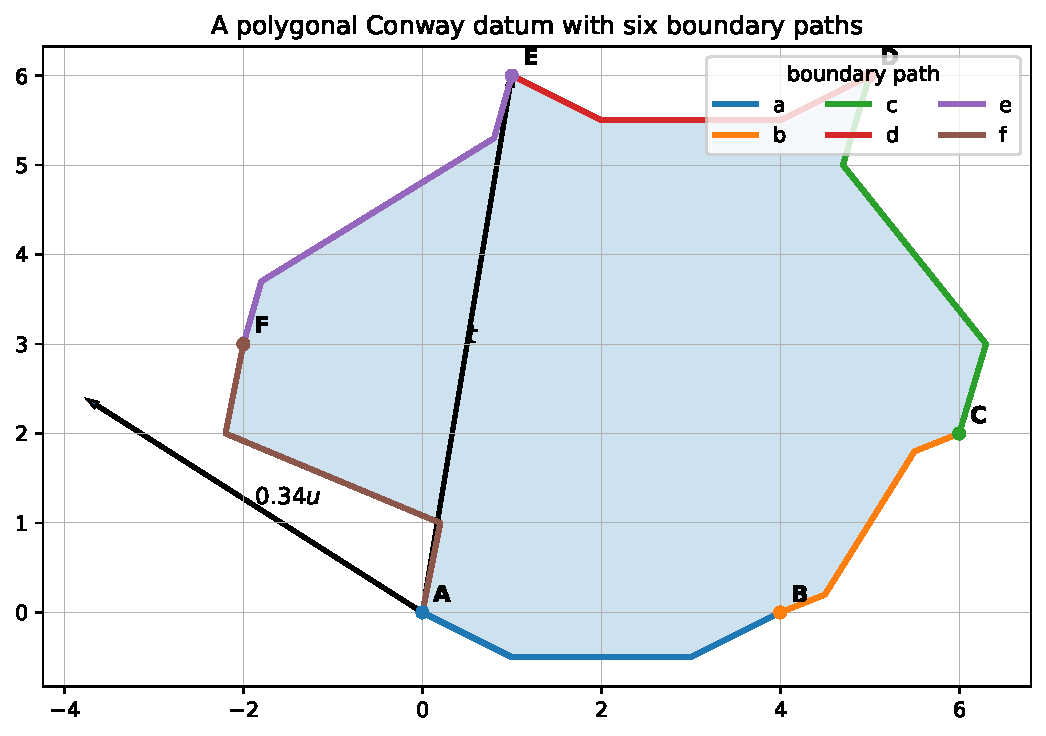
\includegraphics[width=0.91\textwidth]{zigzag_conway_tile.pdf}
\caption{A rational PL Conway datum.  The path \(d\) is the translated reverse of \(a\); each of \(b,c,e,f\) is a two-sided zigzag around its endpoint midpoint.}
\label{fig:exampletile}
\end{figure}

\subsection{Local equations}

The first period is
\[
 t=E-A=(1,6)=D-B.
\]
Adding \(t\) to the vertices of \(a\) gives
\[
 [(1,6),(2,\tfrac{11}2),(4,\tfrac{11}2),(5,6)],
\]
which is exactly \(\rev(d)\).

For \(b\), the doubled center is
\[
 B+C=(10,2).
\]
The half-turn exchanges \((4,0)\leftrightarrow(6,2)\) and
\[
 (\tfrac92,\tfrac15)\leftrightarrow(\tfrac{11}2,\tfrac95).
\]
Thus \(\half{B+C}(b)=\rev(b)\).  The other three paths were chosen in the same paired way, with doubled centers
\[
 C+D=(11,8),\qquad E+F=(-1,9),\qquad F+A=(-2,3).
\]
Every local Conway check is therefore an exact rational equality.

\subsection{Periods and area}

The second period is
\[
 u=E+F-B-C=(-11,7).
\]
Consequently
\[
 \det(t,u)=
 \det\begin{pmatrix}1&-11\\6&7\end{pmatrix}
 =1\cdot7-6(-11)=73.
\]
The shoelace sum of the eighteen effective boundary vertices is also \(73\), so
\[
 \Area(T)=\frac{73}{2}.
\]
The period parallelogram has area \(73\), exactly the area of two tile copies.

The selected half-turn is
\[
 R(x)=E+F-x=(-1,9)-x.
\]
The explicit tiling is therefore
\[
 T+m(1,6)+n(-11,7),
 \qquad
 R(T)+m(1,6)+n(-11,7).
\]
A finite window is shown in \cref{fig:exampletiling}.

\begin{figure}[htbp]
\centering
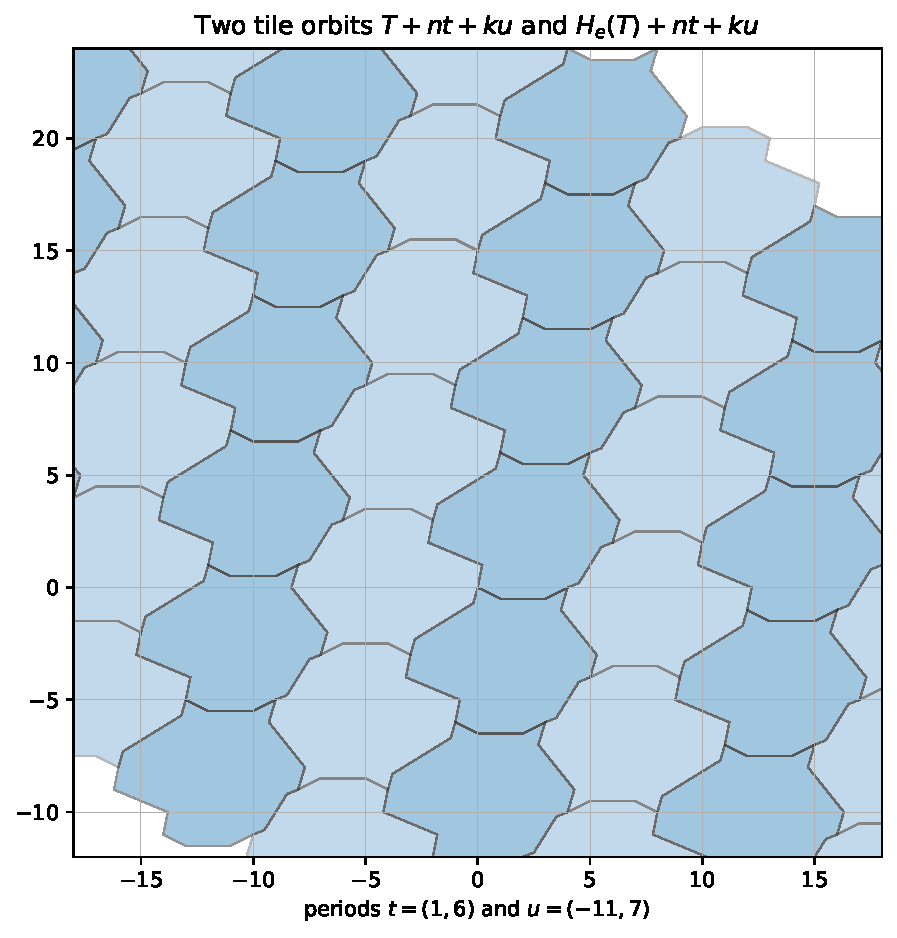
\includegraphics[width=0.88\textwidth]{zigzag_conway_tiling.pdf}
\caption{A window of the two-orbit tiling.  Alternating opacity distinguishes the direct and half-turned translation orbits.}
\label{fig:exampletiling}
\end{figure}

\subsection{Exact executable certificate}

The standard-library Python kernel performs the following checks with \code{fractions.Fraction}:
\begin{enumerate}[label=(\arabic*)]
\item cyclic endpoint continuity, at least three marked points, simplicity, and positive orientation;
\item the translated-pair and four half-turn path equations;
\item the four orbit boundary identities from \cref{lem:orbitpairs};
\item \(\det(t,u)=\PathJ(\partial T)=73\);
\item exact ear triangulation of the polygon;
\item exact conversion of both orbit representatives to lattice coordinates;
\item clipping of every relevant translated triangle to the unit square;
\item total clipped area one and zero positive-area intersection for every pair.
\end{enumerate}

The run produces \(58\) nonzero convex pieces in the unit square.  Their total area is exactly \(1\), and the maximum pairwise intersection area is exactly \(0\).  The generated JSON report is included at
\begin{center}
\code{examples/zigzag\_conway\_tile\_report.json}.
\end{center}

The executable result is independent evidence for the worked example, not a substitute for the universal proof.  Its main value for formalization is that it fixes data formats and exercises the same finite algorithms proposed for \code{BuildTorus}.

\section{Constructive and foundational audit}
\label{sec:audit}

A proof can be finite in appearance while still relying on hidden classical principles.  This section records exactly what the argument uses.

\subsection{Principles used}

\begin{enumerate}[label=(\arabic*)]
\item \textbf{Primitive recursion on finite lists.}  Path sums, triangle sums, normalization, clipping, and graph traversal are bounded folds or recursions.
\item \textbf{Quantifier-free induction.}  This proves loop invariants, telescoping sums, interior-edge cancellation, and propagation along a finite tree.
\item \textbf{Decidable integer and rational comparisons.}  Signs of determinants, segment intersections, and sort order are reduced to natural-number comparisons.
\item \textbf{Finite bounded search.}  Used to select the least available ear, intersection, parent, or unvisited face.  Failure returns a default certificate and is excluded by the correctness premise.
\item \textbf{Intuitionistic logic with explicit witnesses.}  The period vectors, half-turn, triangulation data, lattice shifts, and spanning tree are all computed or supplied as finite data.
\item \textbf{Polynomial equality and cancellation.}  Determinant identities live in the signed-difference ring; positivity permits the final cancellation in natural arithmetic.
\end{enumerate}

\subsection{Principles not used}

\begin{enumerate}[label=(\arabic*)]
\item \textbf{No law of excluded middle for arbitrary propositions.}  Every case split is on a Boolean equality or order test for finite codes.
\item \textbf{No choice.}  Finite selections use least bounded search, yielding explicit indices.
\item \textbf{No compactness or infinite branch argument.}  Periodicity reduces the global problem to one finite torus cell.
\item \textbf{No completeness of the real numbers.}  All coordinates and intersections are rational pairs; all equalities are exact.
\item \textbf{No Jordan curve theorem.}  The input disk property is a finite triangulation certificate.  The conclusion is obtained from a torus subdivision, not from separation by an arbitrary curve.
\item \textbf{No covering-space theorem or fundamental-group computation.}  The role of the torus fundamental class is replaced by \cref{lem:constantmultiplicity}, a dual-tree induction.
\item \textbf{No measure theory.}  ``Area'' is a finite determinant sum.  Additivity follows from oriented edge cancellation.
\item \textbf{No universal primitive-recursive evaluator.}  Every checker and constructor is a fixed symbol.
\end{enumerate}

\subsection{Where positivity enters}

The cycle argument alone gives \(C=k[\Torus]\) for some \(k\in\mathbb N\).  Positivity enters twice:
\begin{enumerate}[label=(\alph*)]
\item the disk triangulation orients every input triangle positively, so the face coefficients are natural coverage counts rather than signed cancellation artifacts;
\item \(\det(t,u)=2\Area(T)>0\) permits cancellation in \cref{eq:kcancel}.
\end{enumerate}
Both facts are witnessed by finite determinant inequalities.  There is no appeal to an abstract positivity cone.

\subsection{Why the torus is safe in iPRA}

The notation \(\R^2/L\) is explanatory.  The formal arithmetic proof need never construct an infinite quotient set.  It uses:
\begin{itemize}
\item the unit rational square in lattice coordinates;
\item side tags recording the identifications \(\alpha=0\sim1\) and \(\beta=0\sim1\);
\item finitely many clipped rational pieces;
\item a finite edge/face incidence table; and
\item integer witnesses for lattice congruence.
\end{itemize}
Thus every use of ``torus'' expands to a finite data structure and decidable relations.

\subsection{Faithfulness to the traditional theorem}

The local hypotheses are exactly the labelled Conway criterion, specialized only in representation: each boundary part is a rational PL path and the tile comes with a rational triangulation.  The output is stronger than mere existence because it gives the periods and placements explicitly.  What is not formalized here is a universal theorem over arbitrary topological embeddings with no finite presentation.  Such a statement is not literally a first-order arithmetic sentence until a representation of continuous objects is chosen.

For an effectively presented curved tile, a separate theorem could assume primitive-recursive names, continuity and inverse-separation moduli, plus finite certificates that the relevant boundary symmetries hold.  The finite torus multiplicity argument should then be recovered by sufficiently fine stable PL approximations, but proving that stability is additional represented-topology work.

\subsection{Verification boundary}

The package distinguishes four levels:
\begin{center}
\begin{tabular}{@{}p{0.22\textwidth}p{0.68\textwidth}@{}}
\toprule
Level & Status \\
\midrule
Mathematical PL proof & Complete in this report. \\
Exact example computation & Executed; seven tests pass and the torus certificate accepts. \\
Lean host blueprint & Supplied, with no admitted facts; not elaborated in this runtime. \\
Object-iPRA derivation & Specified in detail; not yet constructed and kernel-checked. \\
\bottomrule
\end{tabular}
\end{center}
This separation prevents executable evidence or a semantic Lean theorem from being reported as a finished \(\Prf\,\PRA\) proof.

\section{Further research questions}
\label{sec:further}

\begin{enumerate}[label=\textbf{Q\arabic*.},leftmargin=*]
\item \textbf{Smallest object-theory proof.}  What is the smallest complete \(\Prf\,\PRA\) derivation of the PL criterion when measured by normalized Lean term size or by the concise proof-checker metrics used in \code{ConciseIPRA}?  The torus coefficient lemma may admit a very small generic library theorem.

\item \textbf{Avoiding a full arrangement.}  Can the formal proof use only pairwise convex clipping, area additivity, and a finite separation lemma, thereby eliminating explicit face enumeration and dual spanning trees?  Which route produces the simpler proof object?

\item \textbf{A general periodic-cycle principle.}  Formalize a reusable theorem: a finite family of positively oriented rational PL disks whose projected boundaries cancel on a lattice torus and whose total area equals the lattice covolume forms a tiling.  Conway's criterion would then be a short boundary-cancellation corollary.  The same principle may cover generalized parallelogons and other wallpaper-group constructions.

\item \textbf{Other wallpaper groups.}  Replace half-turns by rotations of orders \(3,4,6\) or by glide reflections.  Which local boundary equations imply a finite orbifold cycle of multiplicity one?  A uniform ``orbifold chain certificate'' could subsume several classical tiling criteria.

\item \textbf{Represented curved boundaries.}  Starting from the repository's constructive Jordan framework, identify minimal primitive-recursive moduli ensuring that a curved Conway datum has stable finite PL torus certificates.  Can one avoid a full constructive Schoenflies theorem?

\item \textbf{Automatic criterion discovery.}  Given a rational polygonal tile, use bounded search to find six boundary breakpoints and normalized path correspondences satisfying \code{ConwayOK}.  The search is decidable for a fixed finite subdivision.  What is its complexity, and can symmetry hashing make it practical for large polyforms?

\item \textbf{Certificate minimization.}  The worked example's cutter returns \(58\) convex pieces.  Find a canonical minimal torus subdivision or a proof-producing simplifier that merges adjacent pieces while preserving exact boundary tags.

\item \textbf{Reverse characterization.}  Schattschneider discusses Conway tiles as those admitting suitable \(p2\)-ishedral tilings.  What finite arithmetic hypotheses on a periodic half-turn tiling suffice to reconstruct the six paths and prove the converse in iPRA?

\item \textbf{Degenerate and self-contacting fundamental domains.}  The theorem assumes a disk with simple boundary.  Can the chain method classify when a non-simple generalized parallelogon still yields a legitimate tile after cancellation of retraced arcs?

\item \textbf{Formal proof extraction to graphics.}  Generate SVG or TikZ tiling patches directly from the checked torus certificate, so that the illustration is a verified rendering of the same number-coded data used in the theorem.
\end{enumerate}

\appendix
\section{Algebraic identity sheet}
\label{app:identities}

This appendix collects the equations that a formal development can use as rewrite targets.

\subsection{Endpoint and center equations}

\begin{align*}
 t&=E-A=D-B,\\
 D&=B+t, & E&=A+t,\\
 p&=B+C, & q&=C+D=p+t,\\
 r&=E+F, & s&=F+A=r-t,\\
 u&=r-p=E+F-B-C.
\end{align*}

\subsection{Half-turn compositions}

For \(H_z(x)=z-x\),
\begin{align*}
 H_zH_w&=\tau_{z-w},\\
 H_rH_p&=\tau_u,\\
 H_rH_q&=\tau_{u-t},\\
 H_rH_r&=\mathrm{id},\\
 H_rH_s&=\tau_t.
\end{align*}

\subsection{Boundary equations}

\begin{align*}
 \tau_t(a)&=-d,\\
 H_p(b)&=-b, & H_r(b)&=-\tau_u(b),\\
 H_q(c)&=-c, & H_r(c)&=-\tau_{u-t}(c),\\
 H_r(e)&=-e,\\
 H_s(f)&=-f, & H_r(f)&=-\tau_t(f).
\end{align*}

\subsection{Shoelace equations}

For \(P:X\to Y\),
\begin{align*}
 \PathJ(\tau_wP)&=\PathJ(P)+\det(w,Y-X),\\
 \PathJ(H_zP)&=\PathJ(P)+\det(z,X-Y),\\
 \PathJ(-P)&=-\PathJ(P),\\
 H_{X+Y}P=-P&\Longrightarrow \PathJ(P)=\det(X,Y).
\end{align*}
Thus
\begin{align*}
 \PathJ(a)+\PathJ(d)&=-\det(t,B-A),\\
 \PathJ(b)+\PathJ(c)+\PathJ(e)+\PathJ(f)
 &=\det(B,C)+\det(C,D)+\det(E,F)+\det(F,A),\\
 \PathJ(\partial T)&=\det(t,u)=2\Area(T).
\end{align*}

\section{Primitive-recursive torus constructor}
\label{app:algorithm}

The following pseudocode spells out one total implementation.  Every loop has an explicit finite bound.

\begin{lstlisting}
BuildTorus(code c):
  if not DiskOK(c) or not ConwayOK(c):
      return EmptyCertificate

  t := E(c) - A(c)
  u := E(c) + F(c) - B(c) - C(c)
  delta := det(t,u)
  if delta <= 0: return EmptyCertificate

  triangles := DecodeCertifiedTriangles(c)
  turned := map (x |-> E(c)+F(c)-x) triangles
  pieces := []

  for triangle q in triangles ++ turned:
      q' := map LatticeCoordinates(t,u,delta) q
      I := all integer horizontal shifts whose box meets [0,1]^2
      J := all integer vertical shifts whose box meets [0,1]^2
      for i in I:
        for j in J:
          p := ClipConvex(q' + (i,j), UnitSquare)
          if TwiceArea(p) > 0: append p to pieces

  intersections := all pairwise segment intersections in pieces
  split every edge at its sorted intersection list
  graph := build directed half-edge graph with torus side tags
  faces := bounded face walk from every unused half-edge
  trianglesK := triangulate each rational face
  dualTree := least-search spanning tree of face adjacency
  counts := coverage count of each triangleK by original pieces

  return Certificate(pieces, graph, faces, trianglesK, dualTree, counts)
\end{lstlisting}

The verifier checks:
\begin{enumerate}[label=(\arabic*)]
\item all decoded rational denominators are positive;
\item all segment splits and cyclic face walks are exact;
\item every directed half-edge has the prescribed reverse, including side identifications;
\item every small triangle is positively oriented;
\item the dual tree visits every face exactly once;
\item the boundary coefficient of every edge is zero;
\item adjacent face counts agree; and
\item the common count is one by the determinant-area identity.
\end{enumerate}

A simpler certificate can omit \code{graph}, \code{faces}, and \code{counts}, retaining the clipped convex pieces and checking pairwise zero-area intersections plus total area one.  The report's Python reference uses this variant.  For a first object-theory implementation, the dual-tree form has the advantage that the logical core is just equality propagation on a finite graph.

\section{Object-theory dependency graph}
\label{app:dependencies}

\begin{center}
\begin{tabularx}{\textwidth}{@{}lX@{}}
\toprule
Stage & Depends on \\
\midrule
Point determinant identities & \code{Core.Integers}, \code{Core.LinearAlgebra}, \code{Core.Tactic} \\
Path folds and reversal & \code{Core.Definitions}, \code{Core.Pairing}, quantifier-free induction \\
Path shoelace lemmas & point identities, \code{Core.BoundedSums} \\
Disk boundary cancellation & path folds, triangle incidence certificate \\
Conway period-area theorem & path centrality, translated-pair lemma, disk cancellation \\
Lattice coordinates and clipping & rational arithmetic, \code{Core.Order}, \code{Core.Search} \\
Torus refinement & clipping, finite sorting, pairing/list infrastructure \\
Constant multiplicity & edge incidence, dual spanning tree, induction \\
Multiplicity one & period-area theorem, bounded area sums, positive cancellation \\
Final criterion & all previous stages, propositional composition and universal closure \\
Native export & final \(\Prf\,\PRA\) theorem, \code{pra\_iff\_native} \\
\bottomrule
\end{tabularx}
\end{center}

The dependency graph intentionally keeps topology downstream of exact arithmetic.  This makes failures local: the affine and area theorem can be promoted to the checked derivation library before the full torus constructor is finished.

\section{Theorem and artifact ledger}
\label{app:ledger}

\begin{longtable}{@{}p{0.12\textwidth}p{0.53\textwidth}p{0.25\textwidth}@{}}
\toprule
ID & Claim/artifact & Status \\
\midrule
\endhead
C1 & Composition of half-turns is translation & Proved in \cref{lem:halfturnalgebra}. \\
C2 & Four turned-orbit path identities & Proved in \cref{lem:orbitpairs}. \\
C3 & Open-path shoelace laws & Proved in \cref{lem:Jlaws}. \\
C4 & Central path endpoint determinant & Proved in \cref{lem:Jcentral}. \\
C5 & \(\det(t,u)=2\Area(T)>0\) & Proved in \cref{thm:periodarea}. \\
C6 & Projected two-tile boundary is zero & Proved in \cref{lem:boundaryzero}. \\
C7 & Closed nonnegative top chain has constant multiplicity & Proved in \cref{lem:constantmultiplicity}. \\
C8 & Multiplicity is one & Proved by \cref{eq:kcancel}. \\
C9 & Explicit family tiles the plane & Proved in \cref{thm:mainPL}. \\
P1 & \code{code/conway\_core.py} & Exact rational reference implementation. \\
P2 & \code{code/test\_conway\_core.py} & Seven passing tests at delivery. \\
P3 & Worked torus certificate & \(58\) pieces, exact area \(1\), zero positive-area overlap. \\
L1 & \code{lean/ConwayCriterionBlueprint.lean} & Uncompiled definitions/targets; no admitted facts. \\
L2 & Empty-context \(\Prf\,\PRA\) theorem & Planned, not claimed complete. \\
\bottomrule
\end{longtable}

\section{Reproduction commands}
\label{app:reproduce}

From the package root:

\begin{lstlisting}
(cd code && python3 -m unittest -v test_conway_core.py)
python3 code/conway_core.py examples/zigzag_conway_tile.json \
  --output examples/zigzag_conway_tile_report.json
python3 figures/make_figures.py
bash build.sh
\end{lstlisting}

The exact kernel depends only on the Python standard library.  Figure generation requires Matplotlib.  The PDF build requires a conventional TeX Live installation with the packages in the preamble.

\begin{thebibliography}{99}

\bibitem{Schattschneider1980}
Doris Schattschneider,
``Will It Tile? Try the Conway Criterion!,''
\emph{Mathematics Magazine} 53(4) (1980), 224--233.
\href{https://doi.org/10.1080/0025570X.1980.11976859}{doi:10.1080/0025570X.1980.11976859}.
An updated author-hosted version was also consulted.

\bibitem{Weber2025}
Matthias Weber,
\emph{Games, Graphs, and Groups: An Introduction},
version dated 15 October 2025, Section~3.4, ``Which Shapes Tile?''
\url{https://scholarworks.iu.edu/iuswrrest/api/core/bitstreams/90973f1a-e66f-4a94-9b1a-02bf140c13fc/content}.

\bibitem{GrunbaumShephard1987}
Branko Gr\"unbaum and G.~C. Shephard,
\emph{Tilings and Patterns},
W.~H. Freeman, 1987; Dover reprint, 2016.

\bibitem{Coxeter1969}
H.~S.~M. Coxeter,
\emph{Introduction to Geometry}, 2nd ed.,
Wiley, 1969.

\bibitem{ProveItIPRA}
Vladimir Reshetnikov,
\emph{ProveIt: Primitive Recursive Arithmetic},
repository paths \code{Logic/PrimitiveRecursiveArithmetic/ConciseIPRA} and
\code{Logic/PrimitiveRecursiveArithmetic/Derivations},
commit observed during preparation:
\code{c6643d49ab37d30d1204c689bf7f800db1a04c7b}.
\url{https://github.com/VladimirReshetnikov/ProveIt}.

\bibitem{ProveItJordan}
Vladimir Reshetnikov and contributors,
``A quantitative Jordan curve theorem in iPRA,''
ProveIt research packet
\nolinkurl{Logic/PrimitiveRecursiveArithmetic/docs/proofs/topology/jordan_ipra_constructive_2026-11-15}.

\bibitem{WikipediaConway}
Wikipedia contributors,
``Conway criterion,''
accessed 16 November 2026.
\url{https://en.wikipedia.org/wiki/Conway_criterion}.
Used to confirm the public formulation; mathematical claims in this report are proved independently.

\end{thebibliography}

\end{document}
